% ============================================================
% 第25章 概率初步 — 人教版九年级上册
% 编译命令：xelatex -interaction=nonstopmode 第25章_概率初步.tex
% ============================================================
\documentclass[12pt, a4paper]{ctexart}
\usepackage[margin=2.2cm]{geometry}
\usepackage{amsmath, amssymb}
\usepackage{enumitem}
\usepackage{tcolorbox}
\usepackage{booktabs}
\usepackage{array}
\usepackage{fancyhdr}
\usepackage{xcolor}
\usepackage{tikz}
\usepackage{hyperref}
\usepackage{graphicx}
\usepackage{multirow}
\usepackage{pgfplots}
\pgfplotsset{compat=1.18}

% 颜色定义
\definecolor{mainblue}{RGB}{41, 98, 168}
\definecolor{lightblue}{RGB}{230, 240, 255}
\definecolor{tipgreen}{RGB}{34, 139, 87}
\definecolor{lightgreen}{RGB}{235, 250, 240}
\definecolor{warnred}{RGB}{200, 50, 50}
\definecolor{lightred}{RGB}{255, 240, 240}
\definecolor{examorange}{RGB}{210, 120, 20}
\definecolor{lightorange}{RGB}{255, 248, 235}
\definecolor{apppurple}{RGB}{120, 60, 170}
\definecolor{lightpurple}{RGB}{245, 238, 255}

% 页眉页脚
\pagestyle{fancy}
\fancyhf{}
\fancyhead[L]{\small\textcolor{mainblue}{\textbf{人教版九年级上册 · 第25章 概率初步}}}
\fancyhead[R]{\small\textcolor{mainblue}{概率与统计讲义}}
\fancyfoot[C]{\small —\ \thepage\ —}
\renewcommand{\headrulewidth}{0.6pt}
\renewcommand{\headrule}{\hbox to\headwidth{\color{mainblue}\leaders\hrule height \headrulewidth\hfill}}
\renewcommand{\footrulewidth}{0pt}

% tcolorbox 样式
\newtcolorbox{knowledgebox}[1][]{%
  colback=lightblue, colframe=mainblue,
  fonttitle=\bfseries\large, title=#1,
  arc=3mm, boxrule=0.8pt,
  left=8pt, right=8pt, top=6pt, bottom=6pt
}

\newtcolorbox{tipbox}[1][]{%
  colback=lightgreen, colframe=tipgreen,
  fonttitle=\bfseries, title=#1,
  arc=2mm, boxrule=0.6pt,
  left=6pt, right=6pt, top=4pt, bottom=4pt
}

\newtcolorbox{warnbox}[1][]{%
  colback=lightred, colframe=warnred,
  fonttitle=\bfseries, title=#1,
  arc=2mm, boxrule=0.6pt,
  left=6pt, right=6pt, top=4pt, bottom=4pt
}

\newtcolorbox{examplebox}[1][]{%
  colback=lightorange, colframe=examorange,
  fonttitle=\bfseries, title=#1,
  arc=3mm, boxrule=0.8pt,
  left=8pt, right=8pt, top=6pt, bottom=6pt
}

\newtcolorbox{appbox}[1][]{%
  colback=lightpurple, colframe=apppurple,
  fonttitle=\bfseries, title=#1,
  arc=3mm, boxrule=0.8pt,
  left=8pt, right=8pt, top=6pt, bottom=6pt
}

\setCJKmainfont{Hiragino Sans GB}
\setCJKsansfont{Heiti SC}

\begin{document}

% ============ 标题页 ============
\begin{center}
{\Huge\bfseries\textcolor{mainblue}{第25章\quad 概率初步}}\\[12pt]
{\Large\textcolor{gray}{讲\quad 义}}\\[8pt]
\rule{0.6\textwidth}{1pt}\\[8pt]
{\normalsize 适用：人教版\quad 九年级上册\quad |\quad 课时：4课时}
\end{center}
\vspace{10pt}

% ============ 第一部分：知识点讲解 ============
\section*{\textcolor{mainblue}{一、知识点讲解}}

\subsection*{25.1\quad 随机事件}

\begin{knowledgebox}[1. 确定事件与随机事件]
在一定条件下，某些事件的结果是可以预知的，称为\textbf{确定事件}；某些事件的结果事先无法预知，称为\textbf{随机事件}。

\medskip
\begin{itemize}[leftmargin=2em]
  \item \textbf{必然事件}：在一定条件下，必然会发生的事件。例如：太阳从东方升起。
  \item \textbf{不可能事件}：在一定条件下，不可能发生的事件。例如：掷一枚骰子，朝上的点数为7。
  \item \textbf{随机事件}：在一定条件下，可能发生也可能不发生的事件。例如：掷一枚硬币，正面朝上。
\end{itemize}

\medskip
必然事件和不可能事件统称为\textbf{确定事件}。随机事件发生的可能性有大有小。
\end{knowledgebox}

\begin{warnbox}[易错提醒]
\begin{itemize}[leftmargin=2em]
  \item 判断事件类型时，一定要注意"在一定条件下"这个前提。例如"水往低处流"在地球表面是必然事件，但在太空中就不是。
  \item 随机事件不等于等可能事件。例如"明天会下雨"是随机事件，但下雨和不下雨的可能性通常不相等。
\end{itemize}
\end{warnbox}

\subsection*{25.2\quad 概率的意义}

\begin{knowledgebox}[2. 概率的定义]
\textbf{概率}是衡量随机事件发生可能性大小的量，通常用 $P$ 表示。

\medskip
对于一个随机事件 $A$，我们用 $P(A)$ 表示事件 $A$ 发生的概率。
\begin{itemize}[leftmargin=2em]
  \item $0 \leqslant P(A) \leqslant 1$
  \item 必然事件的概率为 $1$，即 $P(\text{必然事件}) = 1$
  \item 不可能事件的概率为 $0$，即 $P(\text{不可能事件}) = 0$
  \item 随机事件的概率在 $0$ 和 $1$ 之间：$0 < P(A) < 1$
\end{itemize}
\end{knowledgebox}

\begin{tipbox}[规律总结]
概率越大，事件发生的可能性越大；概率越小，事件发生的可能性越小。
当 $P(A)=0.5$ 时，事件 $A$ 发生和不发生的可能性一样大。
\end{tipbox}

\subsection*{25.3\quad 概率的计算——等可能事件}

\begin{knowledgebox}[3. 等可能事件的概率公式]
如果一次试验中，有 $n$ 种等可能的结果，事件 $A$ 包含其中的 $m$ 种结果，那么事件 $A$ 发生的概率为：
\[
  P(A) = \frac{m}{n}
\]
其中 $0 \leqslant m \leqslant n$，因此 $0 \leqslant P(A) \leqslant 1$。
\end{knowledgebox}

\begin{knowledgebox}[4. 列举法求概率]
当试验结果有限且等可能时，可以将所有可能的结果一一列举出来，再统计事件 $A$ 包含的结果数。

\medskip
常用方法：
\begin{itemize}[leftmargin=2em]
  \item \textbf{直接列举法}：适用于结果较少的情况。
  \item \textbf{列表法}：适用于涉及两步试验的情况（如掷两枚骰子）。
  \item \textbf{树状图法}：适用于涉及多步试验的情况，能清晰展示所有可能。
\end{itemize}
\end{knowledgebox}

\begin{warnbox}[易错提醒]
使用概率公式 $P(A) = \dfrac{m}{n}$ 时，必须保证每种结果是\textbf{等可能的}。
例如：掷两个骰子，"点数之和为2"与"点数之和为3"不是等可能事件，不能简单认为概率相同。
\end{warnbox}

\subsection*{25.4\quad 用列表法和树状图求概率}

\begin{knowledgebox}[5. 列表法]
当一次试验涉及\textbf{两个因素}时，可以用表格列出所有可能的结果。

\medskip
\textbf{示例}：同时掷两枚骰子，求点数之和为7的概率。

\medskip
\begin{center}
\begin{tabular}{c|cccccc}
$+$ & 1 & 2 & 3 & 4 & 5 & 6 \\
\hline
1 & 2 & 3 & 4 & 5 & 6 & 7 \\
2 & 3 & 4 & 5 & 6 & 7 & 8 \\
3 & 4 & 5 & 6 & 7 & 8 & 9 \\
4 & 5 & 6 & 7 & 8 & 9 & 10 \\
5 & 6 & 7 & 8 & 9 & 10 & 11 \\
6 & 7 & 8 & 9 & 10 & 11 & 12 \\
\end{tabular}
\end{center}

共有 $6 \times 6 = 36$ 种等可能结果，点数之和为7的有6种，故 $P = \dfrac{6}{36} = \dfrac{1}{6}$。
\end{knowledgebox}

\begin{knowledgebox}[6. 树状图法]
当一次试验涉及\textbf{多个步骤}时，可以用树状图逐层列出所有可能的结果。

\medskip
\textbf{示例}：口袋中有2个红球和1个白球，连续摸两次（不放回），求两次都摸到红球的概率。

\medskip
\begin{center}
\begin{tikzpicture}[
  level 1/.style={sibling distance=4cm, level distance=2cm},
  level 2/.style={sibling distance=1.5cm, level distance=2cm},
  every node/.style={font=\small}
]
\node {开始}
  child {node {红$_1$}
    child {node {红$_2$}}
    child {node {白}}
  }
  child {node {红$_2$}
    child {node {红$_1$}}
    child {node {白}}
  }
  child {node {白}
    child {node {红$_1$}}
    child {node {红$_2$}}
  };
\end{tikzpicture}
\end{center}

共6种结果，两次都红球的有2种，故 $P = \dfrac{2}{6} = \dfrac{1}{3}$。
\end{knowledgebox}

\subsection*{25.5\quad 频率与概率的关系}

\begin{knowledgebox}[7. 频率与概率]
\textbf{频率}：在 $n$ 次重复试验中，事件 $A$ 发生了 $m$ 次，则 $\dfrac{m}{n}$ 称为事件 $A$ 发生的\textbf{频率}。

\medskip
\textbf{频率与概率的关系}：
\begin{itemize}[leftmargin=2em]
  \item 当试验次数较少时，频率波动较大，不能准确反映概率。
  \item 当试验次数较多时，频率会逐渐\textbf{稳定}在概率附近。
  \item 当试验次数足够大时，频率\textbf{趋近于}概率。
\end{itemize}

\medskip
因此，我们既可以用理论计算求概率，也可以用\textbf{大量重复试验的频率}来估计概率。
\end{knowledgebox}

\begin{tipbox}[规律总结]
频率 $\neq$ 概率。频率是试验值，随试验结果变化；概率是理论值，是固定的。
但大量重复试验中，频率会围绕概率上下波动，且波动幅度越来越小。
\end{tipbox}

\subsection*{25.6\quad 几何概型（面积型概率）}

\begin{knowledgebox}[8. 几何概型]
当试验结果与某个\textbf{几何量}（如长度、面积）有关时，可以用几何方法求概率。

\medskip
\textbf{面积型概率公式}：
\[
  P(A) = \frac{\text{事件 } A \text{ 对应的区域面积}}{\text{所有可能结果的总面积}}
\]

\medskip
\textbf{示例}：如图，向一个正方形区域内随机投一点，该点落在阴影区域内的概率为 $\dfrac{S_{\text{阴影}}}{S_{\text{正方形}}}$。
\end{knowledgebox}

\begin{warnbox}[易错提醒]
几何概型要求每个点被选中的可能性是\textbf{均等的}，即"等可能性"。
不能随意对不规则区域使用面积型概率。
\end{warnbox}

\newpage
% ============ 第二部分：例题精讲 ============
\section*{\textcolor{examorange}{二、例题精讲}}

\begin{examplebox}[【例1】判断事件类型]
判断下列事件是必然事件、不可能事件还是随机事件：
\begin{enumerate}[label=(\arabic*)]
  \item 掷一枚均匀硬币，正面朝上；
  \item 从一副扑克牌（52张）中随机抽一张，抽到红桃A；
  \item 任意画一个三角形，其内角和为$180°$；
  \item 掷一枚骰子，朝上的点数大于6。
\end{enumerate}
\end{examplebox}

\textbf{解：}
\begin{enumerate}[label=(\arabic*)]
  \item 随机事件。正面可能朝上，也可能反面朝上。
  \item 随机事件。可能抽到红桃A，也可能抽到其他牌。
  \item 必然事件。三角形内角和定理保证了内角和为$180°$。
  \item 不可能事件。骰子的点数最大为6，不可能大于6。
\end{enumerate}

\begin{examplebox}[【例2】简单等可能事件的概率]
一个不透明袋子里有3个红球和2个白球，这些球除颜色外完全相同。从袋中随机摸出一个球：
\begin{enumerate}[label=(\arabic*)]
  \item 求摸出红球的概率；
  \item 求摸出白球的概率。
\end{enumerate}
\end{examplebox}

\textbf{解：}

袋中共有 $3 + 2 = 5$ 个球，每个球被摸出的可能性相同。
\begin{enumerate}[label=(\arabic*)]
  \item $P(\text{红球}) = \dfrac{3}{5}$
  \item $P(\text{白球}) = \dfrac{2}{5}$
\end{enumerate}

\begin{tipbox}[验证]
$P(\text{红球}) + P(\text{白球}) = \dfrac{3}{5} + \dfrac{2}{5} = 1$，恰好验证了"摸出的球非红即白"。
\end{tipbox}

\begin{examplebox}[【例3】列表法求概率]
同时掷两枚均匀骰子，求：
\begin{enumerate}[label=(\arabic*)]
  \item 点数之和为7的概率；
  \item 点数之和大于9的概率。
\end{enumerate}
\end{examplebox}

\textbf{解：}

用列表法列出所有结果（第一枚骰子为行，第二枚骰子为列），共有 $6 \times 6 = 36$ 种等可能结果。

\begin{enumerate}[label=(\arabic*)]
  \item 点数之和为7的组合有：$(1,6),\;(2,5),\;(3,4),\;(4,3),\;(5,2),\;(6,1)$，共6种。
  \[
    P(\text{和为7}) = \frac{6}{36} = \frac{1}{6}
  \]

  \item 点数之和大于9，即和为10、11、12。
  \begin{itemize}[leftmargin=2em]
    \item 和为10：$(4,6),\;(5,5),\;(6,4)$，共3种
    \item 和为11：$(5,6),\;(6,5)$，共2种
    \item 和为12：$(6,6)$，共1种
  \end{itemize}
  共 $3 + 2 + 1 = 6$ 种。
  \[
    P(\text{和}>9) = \frac{6}{36} = \frac{1}{6}
  \]
\end{enumerate}

\begin{examplebox}[【例4】树状图求概率]
一个不透明盒子中装有2个红球、1个黄球和1个白球，这些球除颜色外完全相同。小明随机摸出两个球（不放回），求：
\begin{enumerate}[label=(\arabic*)]
  \item 两个球颜色相同的概率；
  \item 两个球中至少有一个红球的概率。
\end{enumerate}
\end{examplebox}

\textbf{解：}

将2个红球分别记为红$_1$、红$_2$，用树状图列出摸两个球（不放回）的所有情况。

第一步有4种选择，第二步有3种选择，共 $4 \times 3 = 12$ 种等可能结果。

\begin{enumerate}[label=(\arabic*)]
  \item 两个球颜色相同的情况：
  \begin{itemize}[leftmargin=2em]
    \item 两个红球：(红$_1$,红$_2$)、(红$_2$,红$_1$)，共2种
  \end{itemize}
  \[
    P(\text{颜色相同}) = \frac{2}{12} = \frac{1}{6}
  \]

  \item "至少有一个红球"的对立事件是"两个球都不是红球"。
  两个球都不是红球，即从黄、白中选2个，但只有2个非红球，只能选1对：(黄,白)、(白,黄)，共2种。
  \[
    P(\text{无红球}) = \frac{2}{12} = \frac{1}{6}
  \]
  \[
    P(\text{至少一个红球}) = 1 - \frac{1}{6} = \frac{5}{6}
  \]
\end{enumerate}

\begin{examplebox}[【例5】频率估计概率]
某批产品的合格率为95\%。现从该批产品中随机抽取100件进行检验：
\begin{enumerate}[label=(\arabic*)]
  \item 求恰好有95件合格品的概率（直接写出范围即可）；
  \item 若实际检验中发现有98件合格品，能否说明该批产品的合格率高于95\%？为什么？
\end{enumerate}
\end{examplebox}

\textbf{解：}
\begin{enumerate}[label=(\arabic*)]
  \item 合格率为95\%意味着每件产品合格的概率为0.95。100件中恰好95件合格的概率理论上可以计算（用二项分布），但此处只需知道：由于随机性的存在，不一定恰好是95件，合格数会在95件附近波动。

  \item 不能。因为100次试验属于有限次试验，频率会围绕概率波动。98件合格的频率为0.98，虽然高于0.95，但这可能是正常波动所致，不能仅凭一次100件的检验就断定合格率高于95\%。需要更大的样本量才能更准确地估计。
\end{enumerate}

\begin{examplebox}[【例6】几何概型]
如图所示，正方形 $ABCD$ 的边长为2，分别以四个顶点为圆心、以1为半径画四分之一圆弧，求在正方形内随机取一点，该点落在四个四分之一圆弧围成的阴影区域内的概率。

\begin{center}
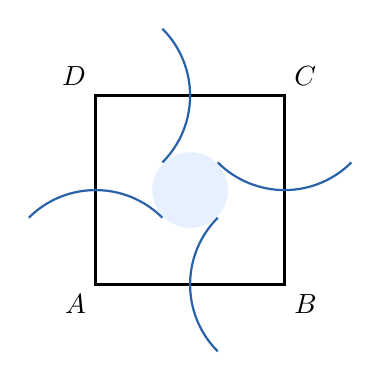
\begin{tikzpicture}[scale=1.2]
  \draw[thick] (0,0) rectangle (2,2);
  \node[below left] at (0,0) {$A$};
  \node[below right] at (2,0) {$B$};
  \node[above right] at (2,2) {$C$};
  \node[above left] at (0,2) {$D$};
  \fill[lightblue] (1,1) circle (0.4);
  \draw[mainblue, thick] (0,0) ++(45:1) arc (45:135:1);
  \draw[mainblue, thick] (2,0) ++(135:1) arc (135:225:1);
  \draw[mainblue, thick] (2,2) ++(225:1) arc (225:315:1);
  \draw[mainblue, thick] (0,2) ++(315:1) arc (315:405:1);
\end{tikzpicture}
\end{center}
\end{examplebox}

\textbf{解：}

正方形面积 $S_{\text{正方形}} = 2^2 = 4$。

四个四分之一圆的面积之和等于一个完整圆的面积：$S_{\text{圆}} = \pi \times 1^2 = \pi$。

设阴影部分面积为 $S_{\text{阴}}$。四个四分之一圆覆盖的区域恰好填充正方形（在四角处），中间的"叶形"区域就是四个圆弧围成的区域。

利用对称性，阴影部分面积 = 正方形面积 $-$ 四个弓形面积，但更直接的方法是：

阴影区域（四叶形）面积 $= S_{\text{正方形}} - 4 \times S_{\text{弓形}}$

其中每个弓形面积 $= S_{\text{正方形}} / 4 - S_{\text{四分之一圆}} = 1 - \dfrac{\pi}{4}$

因此 $S_{\text{阴}} = 4 - 4\left(1 - \dfrac{\pi}{4}\right) = 4 - 4 + \pi = \pi$。

\[
  P = \frac{S_{\text{阴}}}{S_{\text{正方形}}} = \frac{\pi}{4}
\]

\begin{tipbox}[方法总结]
几何概型的关键是正确计算面积（或长度）。本题利用了对称性和面积的加减关系。
\end{tipbox}

\begin{examplebox}[【例7】综合提高——转盘概率]
如图，一个转盘被均匀分成8个扇形区域，其中3个红色、3个蓝色、2个白色。转动转盘一次：
\begin{enumerate}[label=(\arabic*)]
  \item 求指针指向红色区域的概率；
  \item 求指针不指向白色区域的概率；
  \item 小明说"指针指向红色和蓝色的概率一样大"，他说得对吗？请说明理由。
\end{enumerate}
\end{examplebox}

\textbf{解：}
\begin{enumerate}[label=(\arabic*)]
  \item 共8个等可能区域，红色有3个：
  \[
    P(\text{红色}) = \frac{3}{8}
  \]

  \item 白色有2个，非白色有 $8 - 2 = 6$ 个：
  \[
    P(\text{非白色}) = \frac{6}{8} = \frac{3}{4}
  \]

  \item 说得对。红色区域和蓝色区域各占3个，都是8个等可能区域中的3个，所以 $P(\text{红色}) = P(\text{蓝色}) = \dfrac{3}{8}$。
\end{enumerate}

\newpage
% ============ 第三部分：应用题 ============
\section*{\textcolor{apppurple}{三、应用题}}

\begin{appbox}[【应用1】商场抽奖活动]
某商场举行抽奖活动，在一个不透明箱子里放有100张奖券，其中一等奖1张、二等奖4张、三等奖10张，其余为"谢谢参与"。小红随机抽取一张奖券：
\begin{enumerate}[label=(\arabic*)]
  \item 求小红中奖的概率；
  \item 求小红获得三等奖或"谢谢参与"的概率。
\end{enumerate}
\end{appbox}

\textbf{解：}

共100张奖券，"谢谢参与"有 $100 - 1 - 4 - 10 = 85$ 张。
\begin{enumerate}[label=(\arabic*)]
  \item 中奖（一、二、三等奖）共 $1 + 4 + 10 = 15$ 张：
  \[
    P(\text{中奖}) = \frac{15}{100} = \frac{3}{20}
  \]
  \item 三等奖或"谢谢参与"共 $10 + 85 = 95$ 张：
  \[
    P = \frac{95}{100} = \frac{19}{20}
  \]
\end{enumerate}

\begin{appbox}[【应用2】天气预报与决策]
据气象部门统计，某城市6月份下雨的概率为0.3。小明一家计划在6月某天外出郊游：
\begin{enumerate}[label=(\arabic*)]
  \item 求该天下雨的概率；
  \item 如果下雨就取消活动，求活动能正常进行的概率；
  \item 小明连续观察了5天，发现其中4天下雨了。他能否据此认为气象部门的统计数据有误？请用频率与概率的知识分析。
\end{enumerate}
\end{appbox}

\textbf{解：}
\begin{enumerate}[label=(\arabic*)]
  \item $P(\text{下雨}) = 0.3$

  \item 活动正常进行意味着不下雨：
  \[
    P(\text{不下雨}) = 1 - 0.3 = 0.7
  \]

  \item 不能。5天的观察样本量太小，频率 $\dfrac{4}{5} = 0.8$ 与概率 $0.3$ 差异较大，但样本量太小时频率波动幅度大是正常现象。需要长期、大量的数据才能准确估计概率。
\end{enumerate}

\begin{appbox}[【应用3】质量检测]
某工厂生产螺丝钉，已知次品率为2\%。质检部门从一批产品中随机抽取500个进行检验：
\begin{enumerate}[label=(\arabic*)]
  \item 求抽到次品的概率；
  \item 求抽到合格品的概率；
  \item 若在500个产品中实际发现15个次品，由此得到的频率是多少？能否说明该批产品次品率高于2\%？
\end{enumerate}
\end{appbox}

\textbf{解：}
\begin{enumerate}[label=(\arabic*)]
  \item $P(\text{次品}) = 2\% = 0.02$

  \item $P(\text{合格品}) = 1 - 0.02 = 0.98$

  \item 频率 $= \dfrac{15}{500} = 0.03 = 3\%$。虽然 $3\% > 2\%$，但在500次试验中频率围绕概率波动是正常的。3\%与2\%的偏差不算特别大，不能仅凭此断定次品率高于2\%，需要更大样本或统计检验才能下结论。
\end{enumerate}

\begin{appbox}[【应用4】游戏公平性]
小明和小华设计了一个游戏：掷两枚均匀骰子，若点数之和为偶数则小明赢，若点数之和为奇数则小华赢。
\begin{enumerate}[label=(\arabic*)]
  \item 用列表法求点数之和为偶数的概率；
  \item 这个游戏对双方公平吗？为什么？
\end{enumerate}
\end{appbox}

\textbf{解：}

\begin{enumerate}[label=(\arabic*)]
  \item 用列表法（共36种结果）。点数之和为偶数的情形：两数同奇或同偶。
  \begin{itemize}[leftmargin=2em]
    \item 两数同为奇数：第一枚取 $\{1,3,5\}$，第二枚取 $\{1,3,5\}$，共 $3 \times 3 = 9$ 种
    \item 两数同为偶数：第一枚取 $\{2,4,6\}$，第二枚取 $\{2,4,6\}$，共 $3 \times 3 = 9$ 种
  \end{itemize}
  和为偶数共18种。
  \[
    P(\text{偶数}) = \frac{18}{36} = \frac{1}{2}
  \]

  \item $P(\text{奇数}) = 1 - \dfrac{1}{2} = \dfrac{1}{2}$。两人获胜的概率相等，游戏公平。
\end{enumerate}

\newpage
% ============ 第四部分：课堂练习 ============
\section*{\textcolor{tipgreen}{四、课堂练习}}

\begin{enumerate}[label=\textbf{\arabic*.}, leftmargin=2em]
  \item 下列事件中，属于随机事件的是（\quad）。
  \begin{enumerate}[label=A.]
    \item 地球绕太阳公转
    \item 水在标准大气压下加热到$100°C$会沸腾
    \item 从装有3个红球的袋中摸出一个白球
    \item 明天本地最高气温为$35°C$
  \end{enumerate}

  \item 一个不透明袋中装有4个白球和6个黑球，每个球除颜色外完全相同。随机摸出一个球，求：
  \begin{enumerate}[label=(\arabic*)]
    \item 摸出白球的概率；
    \item 摸出黑球的概率。
  \end{enumerate}

  \item 同时抛掷两枚硬币，求：
  \begin{enumerate}[label=(\arabic*)]
    \item 两枚都正面朝上的概率；
    \item 至少一枚正面朝上的概率。
  \end{enumerate}

  \item 一副扑克牌去掉大小王后共52张，随机抽取一张，求：
  \begin{enumerate}[label=(\arabic*)]
    \item 抽到红桃的概率；
    \item 抽到K的概率；
    \item 抽到红桃K的概率。
  \end{enumerate}

  \item 口袋里有3个红球和1个白球，它们除颜色外完全相同。先摸出一个球，记下颜色后放回，再摸出一个球。求两次都摸到红球的概率。

  \item 一个转盘被分成面积相等的3个扇形，分别标为$A$、$B$、$C$。连转两次，用列表法求两次转到的字母不相同的概率。

  \item 在一个边长为4的正方形内随机投一点，求该点到正方形中心的距离小于2的概率。（提示：考虑圆的面积）

  \item 小华做抛硬币试验，抛了10次，有7次正面朝上。他又抛了990次（总共1000次），有496次正面朝上。请解释为什么1000次的频率比10次的频率更接近0.5。
\end{enumerate}

\vspace{10pt}
\begin{knowledgebox}[参考答案]
\begin{enumerate}[label=\textbf{\arabic*.}, leftmargin=2em]
  \item 选D。A为必然事件，B为必然事件，C为不可能事件，D为随机事件。

  \item
  \begin{enumerate}[label=(\arabic*)]
    \item $P(\text{白球}) = \dfrac{4}{10} = \dfrac{2}{5}$
    \item $P(\text{黑球}) = \dfrac{6}{10} = \dfrac{3}{5}$
  \end{enumerate}

  \item 两枚硬币的所有结果：(正,正)、(正,反)、(反,正)、(反,反)，共4种。
  \begin{enumerate}[label=(\arabic*)]
    \item $P(\text{两正}) = \dfrac{1}{4}$
    \item $P(\text{至少一正}) = 1 - P(\text{两反}) = 1 - \dfrac{1}{4} = \dfrac{3}{4}$
  \end{enumerate}

  \item 共52张牌。
  \begin{enumerate}[label=(\arabic*)]
    \item 红桃13张：$P = \dfrac{13}{52} = \dfrac{1}{4}$
    \item K有4张：$P = \dfrac{4}{52} = \dfrac{1}{13}$
    \item 红桃K只有1张：$P = \dfrac{1}{52}$
  \end{enumerate}

  \item 有放回地摸两次，每次有4种可能，共 $4 \times 4 = 16$ 种。两次都红球：$3 \times 3 = 9$ 种。
  $P = \dfrac{9}{16}$。

  \item 共 $3 \times 3 = 9$ 种结果。两次相同：(A,A)、(B,B)、(C,C)共3种。
  $P(\text{不相同}) = 1 - \dfrac{3}{9} = \dfrac{6}{9} = \dfrac{2}{3}$。

  \item 正方形面积 $= 16$，以中心为圆心、半径为2的圆面积 $= 4\pi$。
  $P = \dfrac{4\pi}{16} = \dfrac{\pi}{4}$。

  \item 根据大数定律，试验次数越多，频率越趋近于概率。10次试验太少，频率波动大（0.7）；1000次试验样本量大，频率（0.496）更稳定地接近概率0.5。
\end{enumerate}
\end{knowledgebox}

\vfill
\begin{center}
\small\textcolor{gray}{本讲义仅供教学参考，例题可根据学生水平调整难度。}
\end{center}

\end{document}
